\documentclass{beamer}
\usepackage{graphicx}
\usepackage[utf8]{inputenc}
\usetheme{Warsaw}

\beamertemplatenavigationsymbolsempty 

\title{Manejo de Memoria - Fragmentacion}
\author{Silvio Vileriño}
\date{09 de octubre de 2014}

\begin{document}

\begin{frame}
  \maketitle
\end{frame}

\begin{frame}
  \frametitle{Contexto de la clase}    
  \framesubtitle{Sistemas operativos - Post-Teorica Manejo Memoria}
  \begin{itemize}
    \setlength{\itemsep}{2pt}
    \item Este ejercicio es de la practica 4 de Sistemas Operativos (Manejo de memoria)
    \pause
    \item Clase practica a darse luego de la teorica de Manejo de memoria.
    \pause
    \item Repaso rapido de fragmentacion y algoritmos de asignacion de memoria.
    \pause
    \item El ejercicio elegido para la PO integra los conceptos de fragmentacion y algoritmos de asignacion de memoria.
    \pause
    \item Dejo como tarea buscar un contraejemplo de algo que al principio puede no ser muy intuitivo y es algo que considero importante que los alumnos puedan entender por su cuenta, y de ser necesario pueden venir a consultar luego.
  \end{itemize}
\end{frame}

\begin{frame}
  \frametitle{Uso eficiente de la memoria}    
  \framesubtitle{Fragmentacion}
  La fragmentacion es un fenomeno en el cual el espacio de memoria es usado de forma ineficiente, reduciendo la capacidad y/o la performance del sistema.
  \pause
  \begin{itemize}
    \setlength{\itemsep}{15pt}
    \item \textbf{Fragmentacion interna:} Ocurre cuando un bloque de memoria asignado no es aprovechado en su totalidad
    \pause
    \item \textbf{Fragmentacion externa:} Este fenomeno ocurre cuando la memoria libre total(suma de todos los bloques libres dispersos) es mayor o igual que la memoria requerida por un proceso pero no puede cumplirse al peticion dado que no existe un bloque contiguo de memoria libre de tamaño mayor o igual al requerido.
  \end{itemize}
  \vspace{15pt}
  \pause
  Notar que diferentes tipos de fragmentacion pueden ocurrir al mismo tiempo.
\end{frame}

\begin{frame}
  \frametitle{Uso eficiente de la memoria}    
  \framesubtitle{Algoritmos de asignacion de memoria}
  Consideremos un sistema que utiliza particiones de memoria en bloques de tamaño variable.\\  
  Recordemos rapidamente los algoritmos de asignacion de memoria.
  \begin{itemize}
    \setlength{\itemsep}{7pt}
    \pause
    \item \textbf{First fit:} Elegir el primer bloque disponible para responder la peticion de memoria.
    \pause
    \item \textbf{Best fit:} Recorrer toda la lista de bloques disponibles y elegir el que \textbf{mas} se ajuste a la memoria requerida en la peticion \textbf{minimizando la fragmentacion interna}.
    \pause
    \item \textbf{Worst fit:} Recorrer toda la lista de bloques disponibles y elegir el que \textbf{menos} se ajuste a la memoria requerida en la peticion \textbf{maximizando la fragmentacion interna}.
  \end{itemize}
\end{frame}

\begin{frame}
  \frametitle{Ejercicio 4.3}
  \framesubtitle{Enunciado}
      Se tiene un sistema con 16 MB de RAM que utiliza particiones fijas para ubicar a los programas
      en memoria. 
      \begin{itemize}
          \setlength{\itemsep}{8pt}
          \item Cuenta con particiones de los siguientes tamaños:
          8 MB, 1 MB, 4 MB, 512 KB, 512 KB, 2 MB, en ese orden.
          \item Se desean ejecutar 5 programas de los siguientes tamaños:
          500 KB, 6 MB, 3 MB, 20 KB, 2 MB, en ese orden.
          \item 1. Indique como asignaria las particiones utilizando best-fit. ¿Cual es la cantidad de bytes de memoria desperdiciados?
          \item 2. ¿Alguna de las estrategias de asignacion vistas en clase (peor-ajuste, primer-ajuste) produce como resultado la imposibilidad de ejecutar los 5 programas a la vez?
      \end{itemize}
\end{frame}

\begin{frame}
  \frametitle{Ejercicio 4.3}    
  \framesubtitle{Best fit}
    Veamos que ocurre con la fragmentacion en esta configuracion de la memoria utilizando el algoritmo best fit
    \begin{enumerate}
    \setlength{\itemsep}{5pt}
    \pause
    \item Ubicamos el programa de 500Kb en un bloque de 512Kb, pues es el mas indicado segun el algoritmo best-fit.Aqui tenemos 12 bytes desperdiciados, \textbf{produciendo fragmentacion interna}.
    
    \pause
    \item Ubicamos el programa de 6Mb en un bloque de 8Mb. \textbf{2 Mb se desperdician debido a la fragmentacion interna}.

    \pause
    \item El programa de 3Mb va al bloque de 4Mb libre. \textbf{Nuevamente perdemos 1Mb}.

    \pause
    \item El programa de 20Kb va al bloque de 512Kb libre. \textbf{Desperdiciamos 492Kb}.

    \pause
    \item El programa de 2Mb va al bloque de 2Mb libre. \textbf{Aqui no tenemos fragmentacion interna}.
  \end{enumerate}
  \pause
  \textbf{Tenemos en total 3576 bytes despercidiados.}
\end{frame}

\begin{frame}
  \frametitle{Ejercicio 4.3}
  \framesubtitle{Seguimiento Best fit}
   \begin{figure}[h!]
    \centering        
      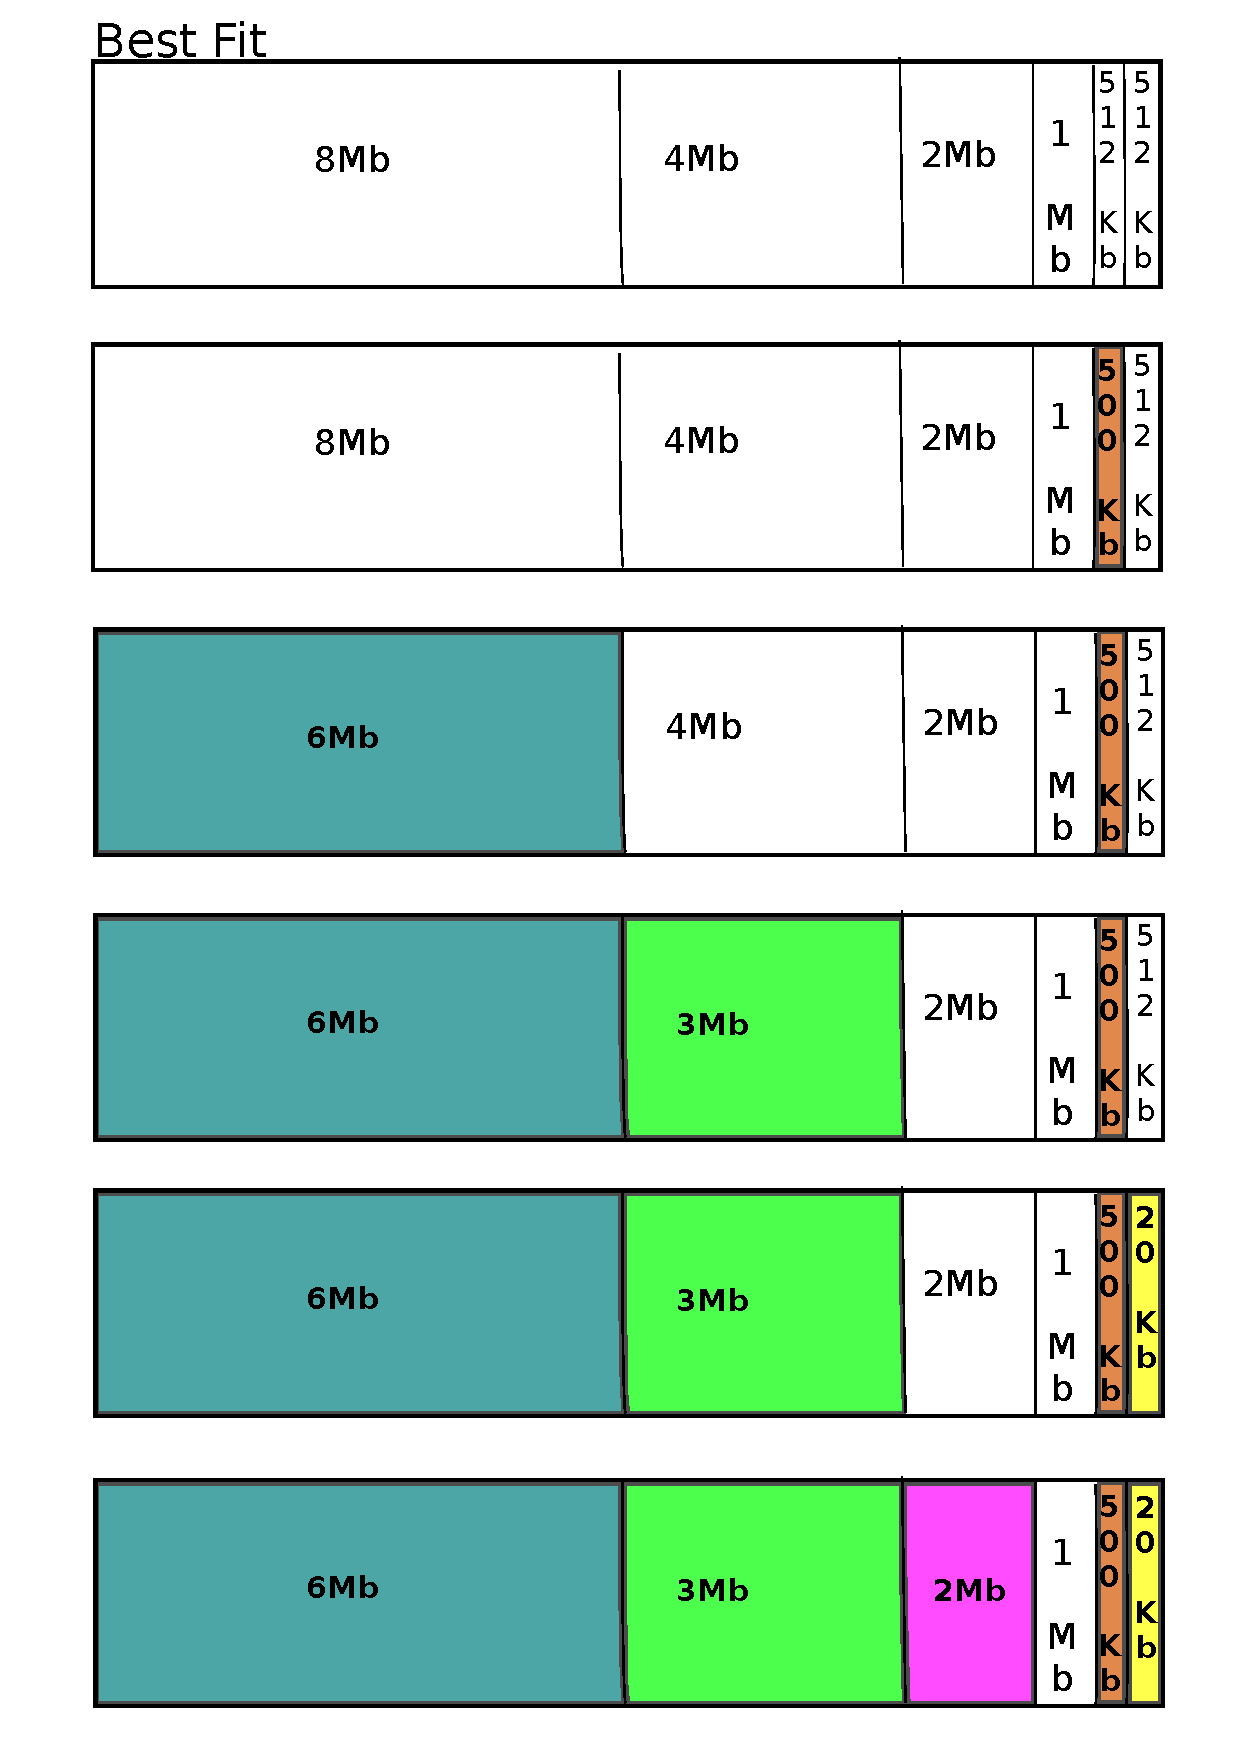
\includegraphics[scale=0.25]{best-fit.pdf}
    \caption{Best Fit}
  \end{figure}
\end{frame}

\begin{frame}
  \frametitle{Ejercicio 4.3}
  \framesubtitle{Seguimiento First Fit}
  La idea es que aca en el pizarron interactue con los alumnos, para resolver el ejercicio entre todos y luego vemos la resolucion.  
   \begin{figure}[h!]
    \centering        
      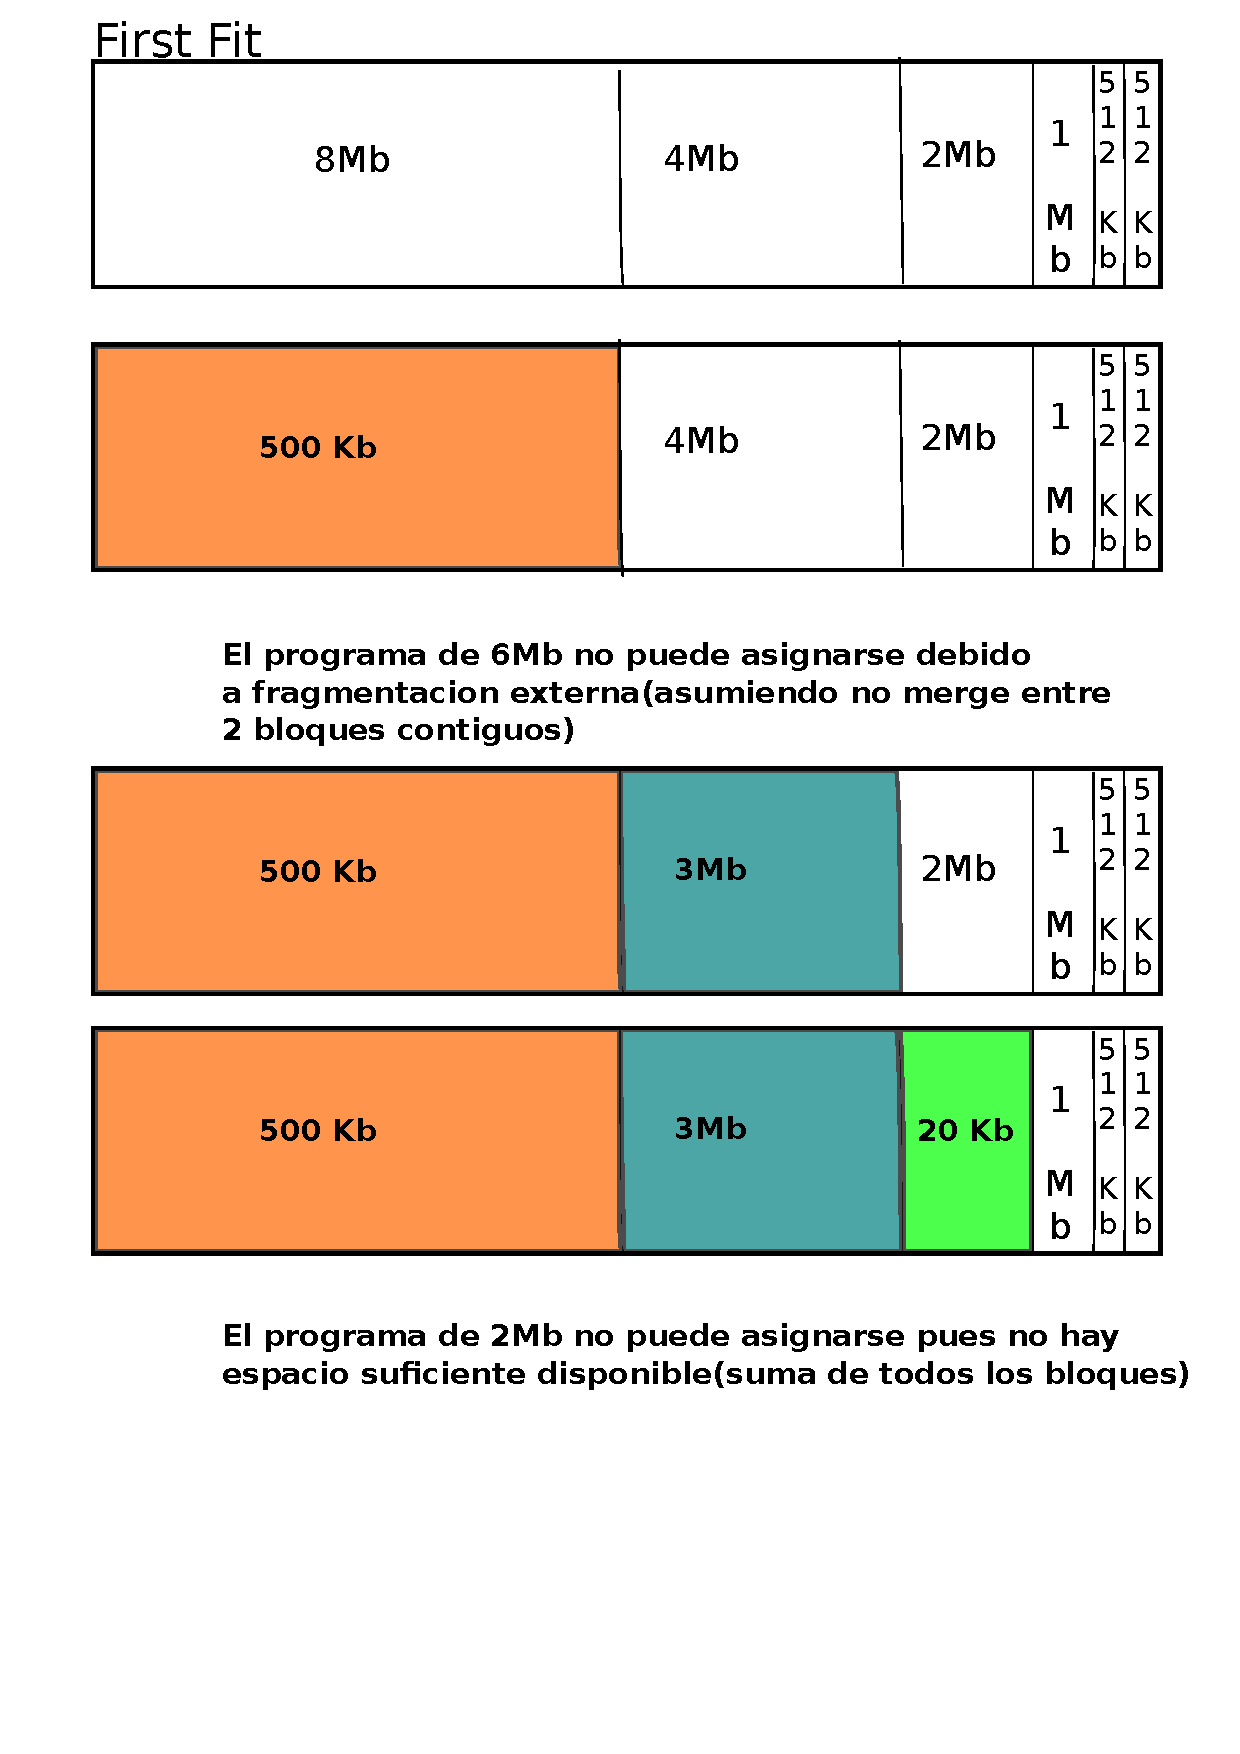
\includegraphics[scale=0.25]{first-fit.pdf}
    \caption{First Fit}
  \end{figure}
\end{frame}

\begin{frame}
  \frametitle{Ejercicio 4.3}    
  \framesubtitle{Seguimiento Worst Fit}
  La idea es que aca en el pizarron interactue con los alumnos, para resolver el ejercicio entre todos y luego vemos la resolucion.
   \begin{figure}[h!]
    \centering        
      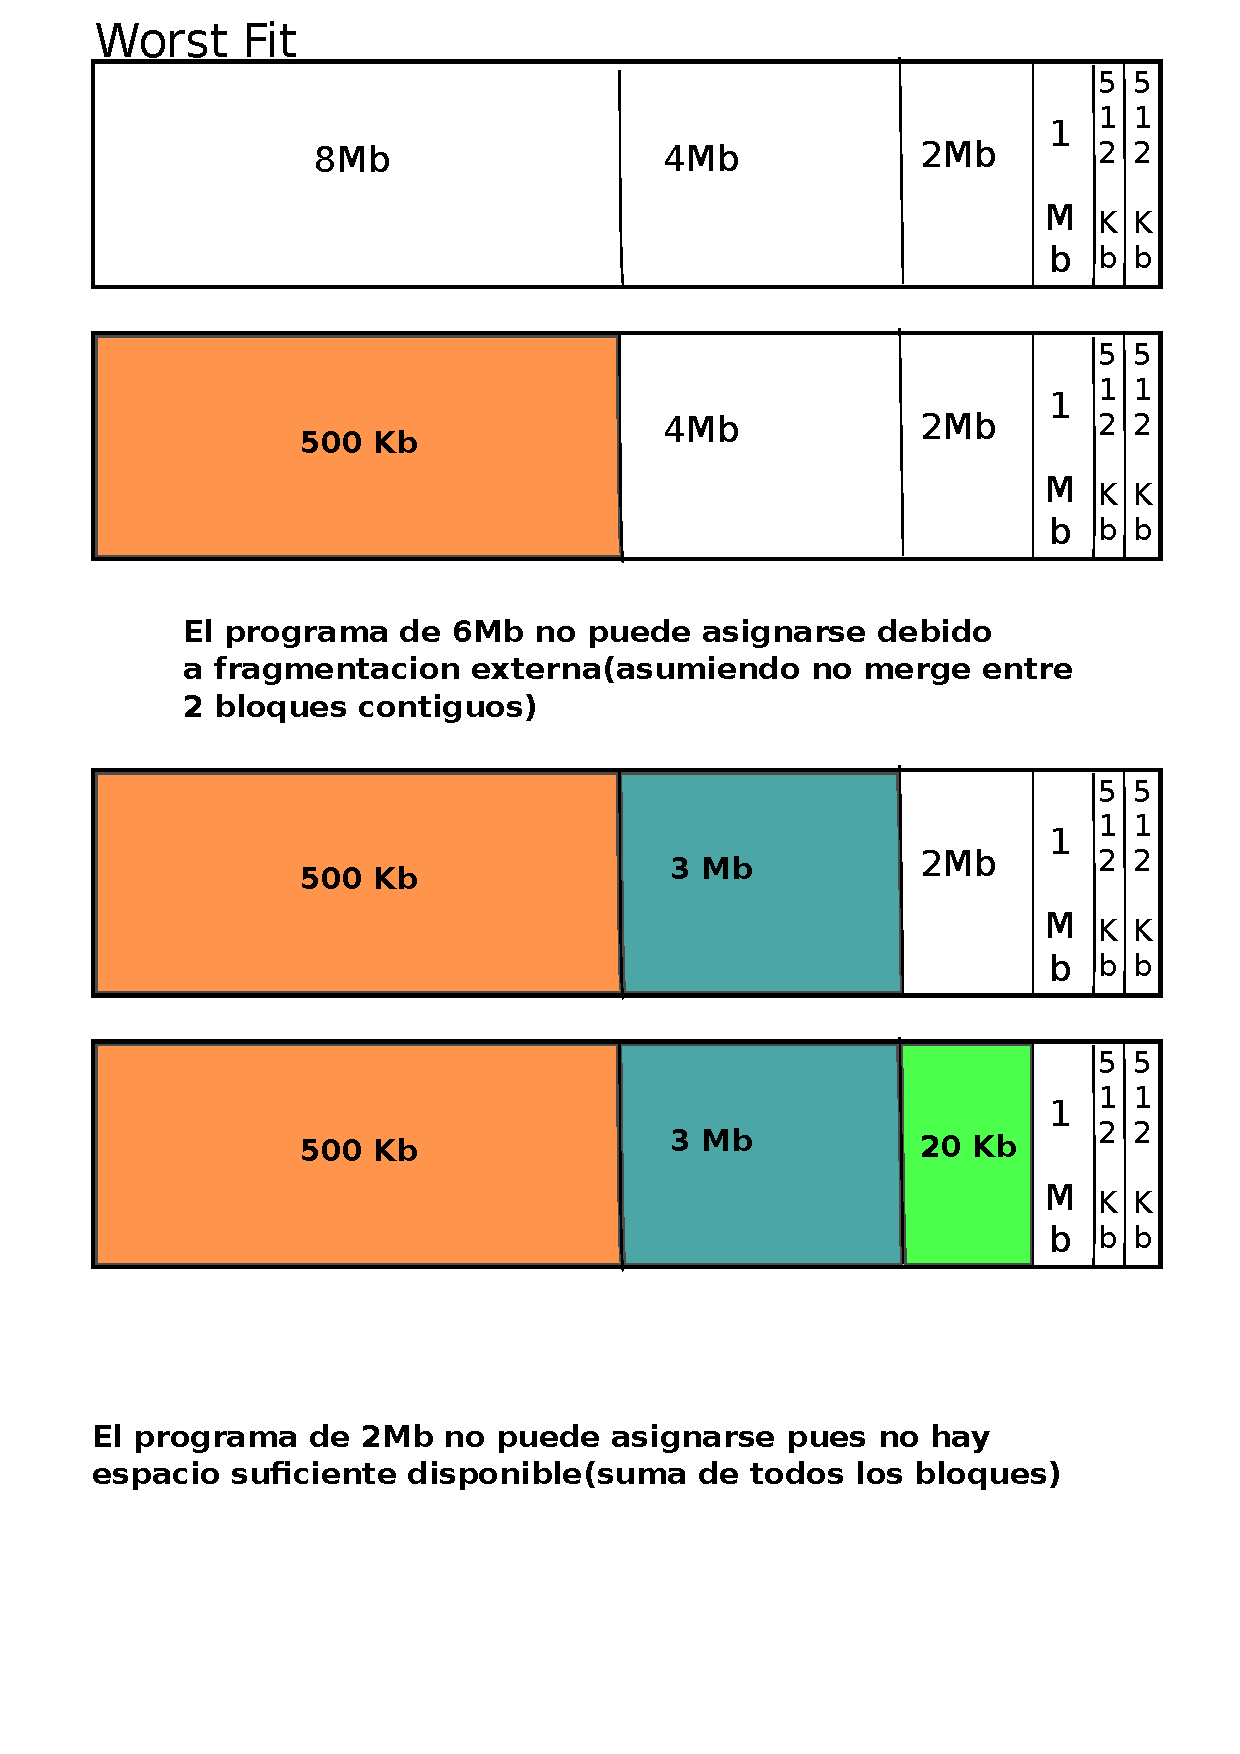
\includegraphics[scale=0.25]{worst-fit.pdf}
    \caption{Worst Fit}
  \end{figure}
\end{frame}

\begin{frame}
  \frametitle{Ejercicio 4.3}    
  \framesubtitle{Continuacion - Conclusion}    
    \begin{enumerate}
    \setlength{\itemsep}{5pt}    
    \item Ya vimos que ocurre con los algoritmos worst-fit y first-fit en las slides anteriores.
    \pause
    \item A diferencia del algoritmo best fit \textbf{en este ejemplo particular}, con los otros algoritmos hay programas que no pueden ser cargados en memoria debido a perdida de memoria por problemas de fragmentacion.
    \pause
    \item Pensar en los tiempos de ejecucion de best-fit/worst-fit versus first-fit.
    \pause
    \item \textbf{Notar que no siempre best fit es el algoritmo que mejor resuelve el problema en todos los casos.} Buscar como tarea un ejemplo de esto.
  \end{enumerate}
\end{frame}

\begin{frame}
  \begin{center}
  \huge ¿Preguntas?
  \end{center}
\end{frame}

\end{document}